\begin{frame}
    \frametitle{Reactor design drives the uranium mass required}
    \begin{columns}
        \column[t]{4.5cm}
            \begin{itemize}
                \item Scenario 5 (MMR + VOYGR) requires the largest average mass of 
                      enriched uranium
                \item Scenario 2 (MMR) requires the largest mass of \gls{HALEU}
                \item Scenario 3 (Xe-100) requires the smallest mass of enriched 
                      uranium
                \item Scenario 5 (MMR + VOYGR) requires the smallest mass of \gls{HALEU}
            \end{itemize}
        \column[t]{5.5cm}
        \vspace{-0.8cm}
            \begin{figure}
                \centering
                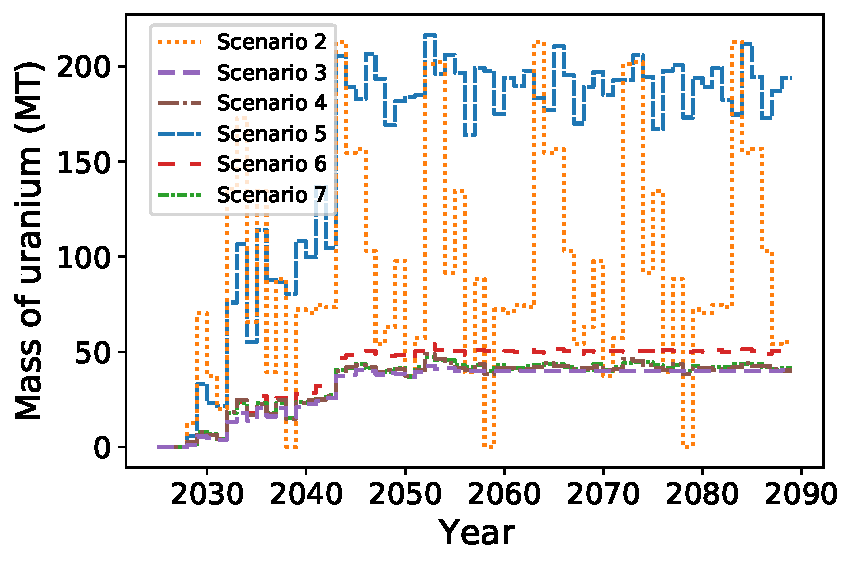
\includegraphics[scale=0.43]{nogrowth_AR_uranium.pdf}
                \caption{Annual average mass of enriched uranium required to fuel
                advanced reactors in Scenarios 2-7.}
                \label{fig:uranium}

        \end{figure}
    \end{columns}
\end{frame}

\begin{frame}
    \frametitle{\gls{SWU} capacity is a function of product mass and assay}
    \begin{columns}
        \column[t]{4.3cm}
            \begin{itemize}
                \item Scenario 2 (MMR) requires the largest average \gls{SWU} 
                \item The other scenarios are comparable for the average 
                      capacity they require
                \item This result does not capture cascade configurations or 
                      facility categories
                
            \end{itemize}
        \column[t]{5.7cm}
        \vspace{-1cm}
        \begin{figure}
                \centering
                \includegraphics[scale=0.43]{nogrowth_AR_swu.pdf}
                \caption{Annual average \gls{SWU} capacity required to produce 
                enriched uranium for and advanced reactors in Scenarios 2-7.}
                \label{fig:swu}
        \end{figure}
    \end{columns}
\end{frame}

\begin{frame}
    \frametitle{\gls{SNF} discharged follows with fuel mass}
    \begin{columns}
        \column[t]{4.3cm}
            \begin{itemize}
                \item Scenario 5 (MMR + VOYGR) discharges the largest mass of \gls{SNF}
                \item Scenario 3 (Xe-100) discharges the least \gls{SNF}
                \item Scenario 2 (MMR) discharges \gls{SNF} the latest
                \item Cumulative masses range between 25,654 MT (Scenario 3) to 
                      112,913 MT (Scenario 5)
                
            \end{itemize}
        \column[t]{5.7cm}
        \vspace{-1cm}
        \begin{figure}
                \centering
                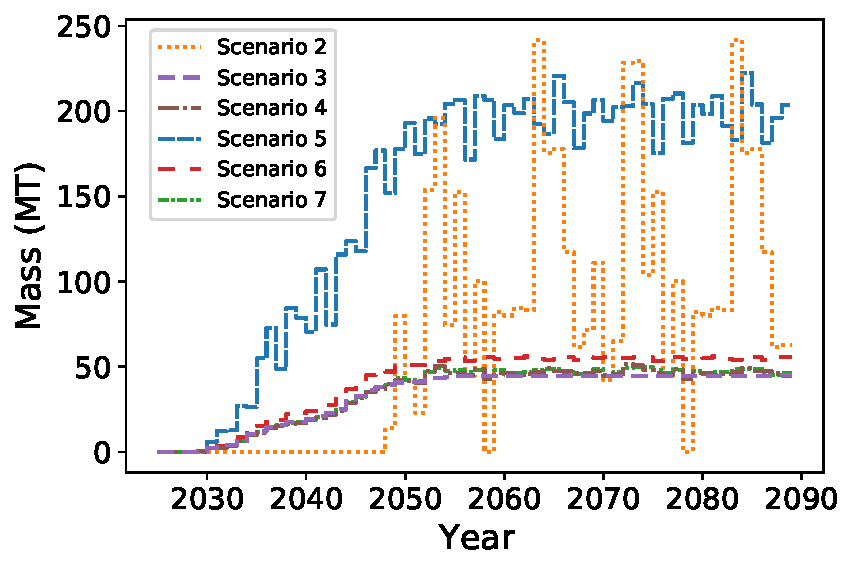
\includegraphics[scale=0.43]{nogrowth_AR_waste.pdf}
                \caption{Annual average mass of \gls{SNF} discharged from 
                advanced reactors in Scenarios 2-7.}
                \label{fig:waste}
        \end{figure}
    \end{columns}
\end{frame}
